
\centerline{\textbf{ \LARGE Threads}}


% ----------------------------------------------------------------------------


\begin{enumerate}

  \item Segments of a program: code, data, PCB, stack if needed
  \item PCB contains all the information of the process ex. P-id, priority
  \item Context switching is faster in threads.

  \begin{figure}[h]
      \centering   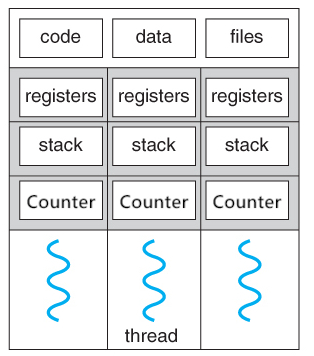
\includegraphics[scale=2]{./images/threads_01.jpeg}
  \end{figure}

  \item Threads
    \begin{enumerate}
      \item Threads share code, data, files with parent process
      \item Each thread have separate stack, PC and registers.
    \end{enumerate}

  \item Types of thread : user and kernel

  \begin{myTableStyle}
    \begin{tabular}{ |m{8cm}|m{8cm}| } \hline
        User thread                                 &     Kernel Thread                                   \\ \hline
        Implemented by user                         &     Implemented by OS.                              \\ \hline
        created and scheduled using thread library  &     created and scheduled by the kernel             \\ \hline
        Not recognize by OS                         &     Recognized by OS.                               \\ \hline
        Managed by user process                     &     Threads and process are managed by OS           \\ \hline
        share the same address space                &     Have separate address space                     \\ \hline
        Independent of OS. Portable                 &                                                     \\ \hline
        Faster thread switching                     &     Thread switching requires system calls          \\ \hline
        threads decide when to give control to other&     CPU can be take from a process forcefully       \\ \hline
        IO request will block whole process         &     OS will schedule another thread                 \\ \hline
        Can not be scheduled independently          &     Multiple threads of same process can be scheduled on different cpu          \\ \hline
        Faster, easy implementation, no hardware support needed&            \\ \hline
    \end{tabular}
  \end{myTableStyle}
  \vspace{0.08in}

\end{enumerate}

% ----------------------------------------------------------------------------

% ----------------------------------------------------------------------------

% ----------------------------------------------------------------------------

% ----------------------------------------------------------------------------

% ----------------------------------------------------------------------------

% ----------------------------------------------------------------------------

% ----------------------------------------------------------------------------

% ----------------------------------------------------------------------------
